\documentclass[10pt]{article}
\usepackage[spanish]{babel}
\usepackage{graphicx}
\usepackage{tabularx} % para width table
\usepackage[left=1.5cm,top=2.4cm,right=2.1cm,bottom=3cm,bindingoffset=0.5cm]{geometry} % original[22 iz,24 arri]
\usepackage{multirow}
\graphicspath{{img/}{img2/}}
\usepackage{url}
\usepackage{amsmath}
\usepackage{hyperref} % Hipervinculos
\usepackage{ragged2e} % Alineación
\usepackage{amssymb} %therefore
\usepackage{float} %Here
\usepackage{listings}
\usepackage{mathrsfs,mathtools} 
\usepackage{pdfpages} %Incluir pdf
\usepackage{csvsimple} %%----------ARCHIVOS CVS


\newsavebox\foobox
\newlength{\foodim}
\newcommand{\slantbox}[2][0]{\mbox{%
        \sbox{\foobox}{#2}%
        \foodim=#1\wd\foobox
        \hskip \wd\foobox
        \hskip -0.5\foodim
        \pdfsave
        \pdfsetmatrix{1 0 #1 1}%
        \llap{\usebox{\foobox}}%
        \pdfrestore
        \hskip 0.5\foodim
}}
\def\Laplace{\slantbox[-.45]{$\mathscr{L}$}}



%% paquetes para esta práctica (aquí abajo)-------------------------------

\usepackage{titlesec}
\titleformat{\section}
{\normalfont\Large\bfseries \raggedright}{\thesection}{1em}{}


%% Preambulo configuraciones adicionales----------------------------------

\newcommand{\iu}{{i\mkern1mu}} % definicon nuevo comando
\addtolength{\jot}{1em} % espacio vertical ecuaciones


%% Cuerpo principal-------------------------------------------------------

\begin{document}
	
	\centering
	\begin{tabular}{ |	p{30 mm}|	p{61 mm}	|	p{33mm}	| p{43mm}	| } 
		\hline
		
		
		\multirow{4}{30mm}{\centering 
\includegraphics[scale=0.22]{logo}} &
		\multirow{4}{61mm}{\centering \textbf{ \textbf{Manual de prácticas del Laboratorio de Análisis de Sistemas y Señales}}}    & Código: & MADO-76 \\
		\cline{3-4}
		& &  Versión & 01 \\
		\cline{3-4}
		& & Página: & 77/97 \\ \cline{3-4}
		& & Sección ISO: & 8.3 \\ \cline{3-4}
		& & Fecha de emisión: & 28 de frebrero 2019 \\
		\hline
	\end{tabular}
\begin{tabular}{ |	c |	c	| } 
	
	\multirow{2}{65mm}{ \centering Facultad de ingeniería} &
	\multirow{2}{111mm}{\centering \textbf{ Area/Departamento: \\ Laboratorio de control y robótica}}   \\
	& \\ \hline
\end{tabular}
\begin{tabular}{|p{180mm}|}
	\multirow{1}{180mm}{ \centering La impresion de este documento es una copia no controlada }  \\ \hline \end{tabular} \\

\vspace{1cm}


{\centering \LARGE Práctica N◦5 Respuesta de Sistemas Dinámicos }

\vspace{1.5cm}

\begin{figure}[!h]
	\centering
	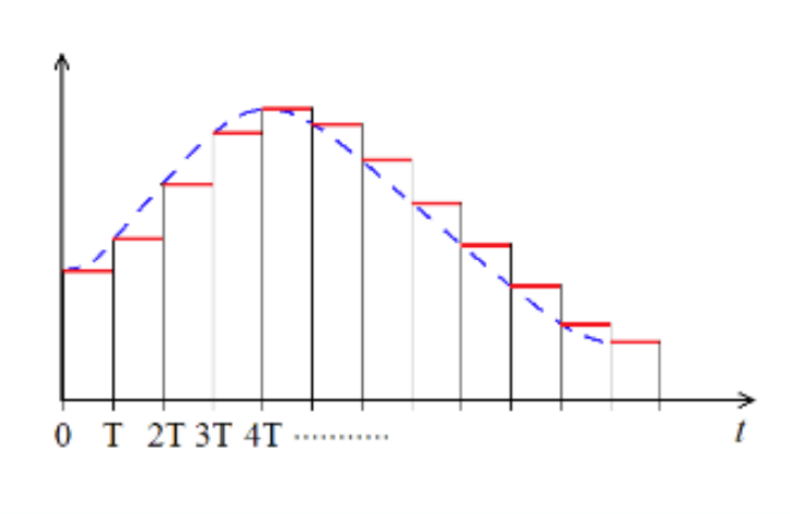
\includegraphics[scale=0.6]{portada.png}
\end{figure}

\hspace{2cm}

\hspace{1cm}
\begin{tabular}{|c| p{122mm}|}
	\hline
	\multirow{4}{50mm}{\\ \centering \large Apellidos y nombres}	 &  \\  
	& Alfaro Domínguez Rodrigo  \\  \cline{2-2}
	&  \\  
	& Barrera Peña Víctor Miguel \\  \cline{2-2}
	&  \\  
	& Villeda Hernández Erick Ricardo \\ 
	\hline
\end{tabular}
\begin{tabular}{|p{50mm} | c | p{80mm}| p{23mm} |}
	Grpo: & 4 & \multirow{2}{90mm}{Profesor: M.I Lauro Fernando Vazquez Alberto } & Calificación \\ \cline{1-2}
	Brigada: & 1 &  &\\ \hline
	Semestre: & 2021-1 & Fecha de ejecución: 29/09/2020 & \\ \hline
\end{tabular}





	\includepdf[pages={2-12}]{latex/practica3.pdf}
	%\noindent \justifying

\section{Previo}

\subsection{Identificar un sistema dinámico que se tenga en casa y definir la salida y la entrada del mismo (para discusión en clase)}
\subsection{¿Como analizaría un sistema de orden mayor?}
Para analizar un sistema de orden superior empezamos por escribir su función de transferencia:
\begin{equation}
H(s)=K\frac{(s-z_1)(s-z_2)...(s-z_n)}{(s-p_1)(s-p_2)(s-p_n)}
\end{equation} 
La mayor parte de la información de como funciona el ssitema nos la darán la localización de los polos y ceros. Esto determina si el sistema es estable o no.\\
En caso de tener polos reales la ecuación toma la siguiente forma:
\begin{equation}
H(s)=\frac{a_1}{s-p_1}+...+\frac{a_n}{s-p_n}
\end{equation}
A partir de aquí analizamos su respuesta a un impulso y un escalón, quedándonos sus ecuaciones de una de las siguientes formas respectivamente:
\begin{equation}
y_{imp}=\alpha_1 e^{p_1t}+..+\alpha_n e^{p_nt}
\end{equation}
\begin{equation}
y_{step}=\beta_0 + \beta_1 e^{p_1t}+...+ \beta_n e^{p_nt}
\end{equation}
Cada polo real p genera un término exponencial en la respuesta. El comportamiento de las osilaciones va a depender de si la parte real del poplo es negativa o positiva, mientras que la magnitud depende de los ceros.\\
En el caso de un sistema de segundo orden podemos escribir su ecuación característica en términos de zeta y omega, de la siguiente forma:
\begin{equation}
\frac{d^2y(t)}{dt^2}+2\zeta \omega_n \frac{dy(t)}{dt}+(\omega_n)^2y(t)=k(\omega_n)^2x(t)
\end{equation}
A partir de su respuesta en la ecuación homogénea podemos llegar a un polinimio de la siguiente forma:
\begin{equation}
s^2+2\zeta\omega_ns+\omega^2_n=0
\end{equation}
La respuesta del sistema va a depender de los valores que tenga el término $\zeta$, siendo sus valores posibles entre cero e infinito positivo. Lo que nos interesará para el diseño de un sistema es que su valor sea mayor o igual a uno.
\subsection{¿Cuál es la importancia de la constante de tiempo $\tau$ y el factor de amortiguamiento $\zeta$ ?}


	\includepdf[pages={13}]{latex/practica3.pdf}
	
\subsubsection{Solución}
 
\textbf{Solución analítica del circuito:}

Empezamos por la sustitución de los valores dados en el ejercicio, donde $\frac{R}{L}=1$ y $\frac{1}{LC}=5$. Con esto podemos reescribir nuestra ecuación de la siguiente forma:

\begin{equation}
	\frac{d^2V_c(t)}{dt^2}+\frac{dV_c(t)}{dt}+5V_g(t)=5V_g(t)
\end{equation}

\noindent Realizamos la sustitución de $V_c(t)=y(t)$ y $V_g(t)=x(t)$

\begin{equation}
	\frac{d^2y(t)}{dt^2}+\frac{dy(t)}{dt}+5y(t)=5x(t)
\end{equation}

\noindent Con dichos cambios ya podemos empezar a aplicar la transformada de Laplace a ambos lados de la ecuación

\begin{equation}
	\Laplace\{{\frac{d^2y(t)}{dt^2}+\frac{dy(t)}{dt}+5y(t)}\}=\Laplace\{{5x(t)}\}
\end{equation}

\begin{equation}
	s^2Y(s)+sY(s)+5Y(s)=5X(s)
\end{equation}

\noindent Factorizamos $Y(s)$ y $X(s)$

\begin{equation}
	Y(s)(s^2+s+5)=5X(s)
\end{equation}

\noindent Si reacomodamos la expresión finalmente llegamos a la función de transferencia

\begin{equation}
	H(s)=\frac{Y(s)}{X(s)}=\frac{5}{(s^2+s+5)}
\end{equation}

\noindent Si consideramos la entrada un escalón, es decir que $X(s)=1$ simplificamos la expresión a 

\begin{equation}
	Y(s)=\frac{5}{(s^2+s+5)}
\end{equation}

\noindent Una vez teniendo la transformada de Laplace podemos aplicar la antitransformada para llegar a la ecuación solución del sistema.

\begin{equation}
	\Laplace^-1\{Y(s)\}=\Laplace^-1\{\frac{5}{(s^2+s+5)}\}
\end{equation}

\begin{equation}
	y(t)=\frac{10\sqrt(19)e^\frac{-t}{2}sin(\frac{\sqrt(19)t)}{2})}{19}
\end{equation}

\noindent\textbf{Representación grafica: }



\begin{figure}[H]
	\centering
	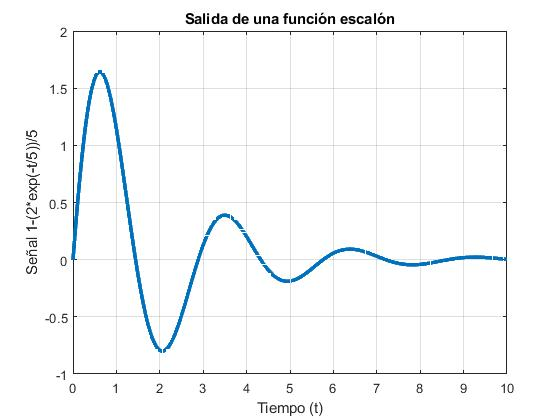
\includegraphics[width=0.7\linewidth]{salidaejercicio1}
	\caption{Gráfica de la función muestreada}
	\label{fig:salidaejercicio1}
\end{figure}

	\includepdf[pages={14}]{latex/practica3.pdf}
	\subsubsection{solución}
\begin{itemize}
\item Considerando un periodo de muestreo de $ T_s = 1 $ y utilizando el método de discretización [...] punto decimal hasta $T_s = 0,0001$).
\end{itemize}

Empezaremos por encontrar la ecuación en diferencias. Para esto tendremos que utilizar la definición que nos permite transformar de una ecuación diferencial a una en diferencias:

\begin{equation}
\frac{dy}{dx}=\frac{y(t)-y(t-T_s)}{T_s}
\end{equation}

\noindent e igualmente usaremos la que nos permite pasar de una diferencial de segundo grado a su equivalente en diferencias:

\begin{equation}
\frac{d^2y}{dt^2)}=\frac{y(t)-2y(t-T_s)+y(t-2T_s}{T_s^2}
\end{equation}

\noindent Tras sustituir ambas definiciones llegamos a:

\begin{equation}
\frac{V_c(t)-2V_c(t-T_s)+V_c(t-2T_s)}{T_s^2}+\frac{R}{L}\frac{V_c(t)-V_c(t-T_s)}{T_s}+\frac{1}{LC}V_c(t)=\frac{1}{LC}V_g(t)
\end{equation}

\noindent Aplicamos las equivalencias que nos dieron al inicio de la práctica $\frac{R}{L}=5$, $\frac{1}{LC}=5$, $V_c(t)=y(t)$ y $V_g(t)=x(t)$

\begin{equation}
\frac{y(t)-2y(t-T_s)+y(t-2T_s)}{T_s^2}+\frac{y(t)-y(t-T_s)}{T_s}+5y(t)=5x(t)
\end{equation}

\noindent \textbf{Salida con $T_s=1$}

\begin{figure}[H]
\centering
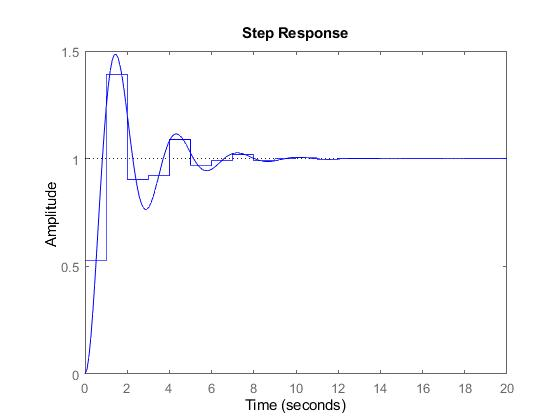
\includegraphics[width=0.7\linewidth]{SalidaTs1}
\caption{Salida con $T_s=1$}
\label{fig:salidaTs1}
\end{figure}

\noindent \textbf{Salida con $T_s=0,0001$}

\begin{figure}[H]
\centering
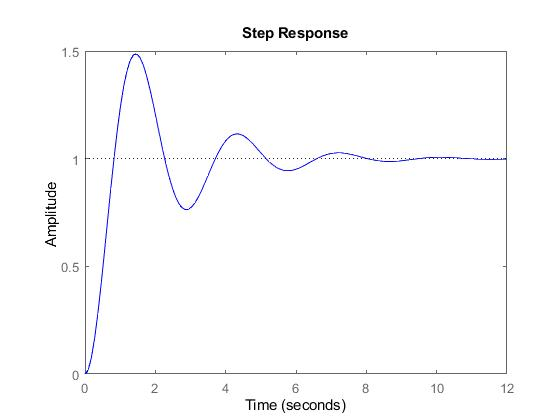
\includegraphics[width=0.7\linewidth]{SalidaTs00001}
\caption{Salida con $T_s=0,0001$}
\label{fig:salidaTs01}
\end{figure}

Para la obtención de las gráficas anteriores se usaron los siguientes comandos de Matlab:

\begin{itemize}
\item Ts=1
\item Hs=tf([5],[1 1 5])
\item Hz=c2d(Hs,Ts,'foh')
\item step(Hs,'-',Hz,'-')
\end{itemize}


Como podemos concluir de observar ambas gráficas, la importancia de $T_s$ radica en que mientras más se acerque su valor a cero mejor será la aproximación de la solución de ecuaciones por diferencias a la solución de la ecuación en tiempo continuo. Esto mismo lo podemos ver al hacer $T_s=0.0001$ parece que las gráficas se sobreponen, mientras que en $T_s=1$ se ve claramente la diferencia entre ambas gráficas. Cabe aclarar que la gráfica obtenida mediante la solución de diferencias finitas nunca va a ser la misma que la de tiempo continuo sin importar cuanto se disminuya $T_s$

\begin{itemize}
	\item Obtenga la función de transferencia del sistema de tiempo continuo.
	\item Utilizando $ T_s = 1 $:
\end{itemize}

\begin{equation}
	H(s)=\frac{Y(s)}{X(s)}=\frac{5}{(s^2+s+5)}
\end{equation}


\textbf{A)} Obtenga la función de transferencia de tiempo discreto de la ecuación en diferencias que resultó en	el punto anterior.

A partir de la ecuación obtenida en el ejercicio anterior

\begin{equation}
	\frac{y(t)-2y(t-T_s)+y(t-2T_s)}{T_s^2}+\frac{y(t)-y(t-T_s)}{T_s}+5y(t)=5x(t)
\end{equation}

Podemos llegar a que si $T_s=1$ nuestra ecuación por diferencias es la siguiente:



\begin{equation}
	\frac{0.5252z^2+1.231z+0.3053}{z^2 +0.6936x + 0.3679}
\end{equation}

Dicha ecuación es obtenida en Matlab tras usar los siguientes comandos.

\begin{itemize}
	\item Ts=1
	\item Hs=tf([5],[1 1 5])
	\item Hz=c2d(Hs,Ts,'foh')
\end{itemize}

\textbf{B)}  Obtenga la función de transferencia de tiempo discreto a partir de la función de transferencia de tiempo continuo del sistema utilizando un diferenciador discreto, ¿cómo son las funciones de transferencia obtenidas en este punto y el anterior? ¿qué puede concluir?

Como ya habíamos mencionado antes, la función de transferencia en tiempo discreto utilizando un diferenciador discreto es la siguiente:

\begin{equation}
	\frac{0.5252z^2+1.231z+0.3053}{z^2 +0.6936x + 0.3679}
\end{equation}

La comparación entre la obtención de la función de transferencia con y sin diferenciador se ve en las gráficas de la siguiente pregunta. Lo que se puede observar es que mediante el uso del diferenciador, la ecuación y su gráfica se acercan más a la ecuación y gráfica de la respuesta en tiempo continuo, es decir, la presencia del diferenciador hace más exacta la aproximación en tiempo discreto.
	\includepdf[pages={15}]{latex/practica3.pdf}
	
\begin{itemize}
	\item Grafique en una sola figura la respuesta al impulso del sistema de tiempo continuo, y las dos aproximaciones
	de tiempo discreto.
\end{itemize}

Para esto se generaron dos gráficas: una sin diferenciador discreto y una con diferenciador discreto, siendo representadas por las curvas roja y amarilla respectivamente. Cabe mencionar que las curvas son la respuesta al impulso.

\noindent \textbf{Salida con $T_s=1$}

\begin{figure}[H]
	\centering
	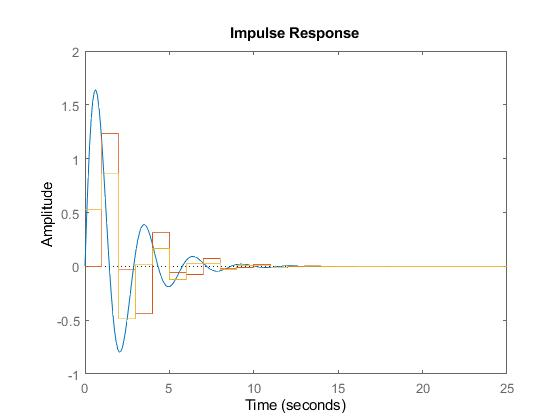
\includegraphics[width=0.7\linewidth]{SalidaTs1DosHz}
	\caption{{Salida con $T_s=1$}}
	\label{fig:salidaTs01-1}
\end{figure}



La obtención de la gráfica anterior se realizó con la siguiente serie de comandos

\begin{itemize}
\item Ts=1
\item Hs=tf([5],[1 1 5])
\item Hz=c2d(Hs,Ts)
\item Hz2=c2d(Hs,Ts,'foh')
\item impulse(Hs)
\item hold on
\item dimpulse(Hz,Ts)
\item hold on
\item dimpulse(Hz2,Ts)
\end{itemize}

\begin{itemize}
	\item Disminuya el tiempo de muestreo hasta obtener una aproximación adecuada de la respuesta del sistema
	y grafique la comparación. ¿Qué aproximación resultó mejor?
\end{itemize}

Para obtener una aproximación adecuada se disminuyó el valor de $T_s$ a 0.0001, generando la siguiente 
\newline

\noindent \textbf{Salida con $T_s=0.0001$}

\begin{figure}[H]
	\centering
	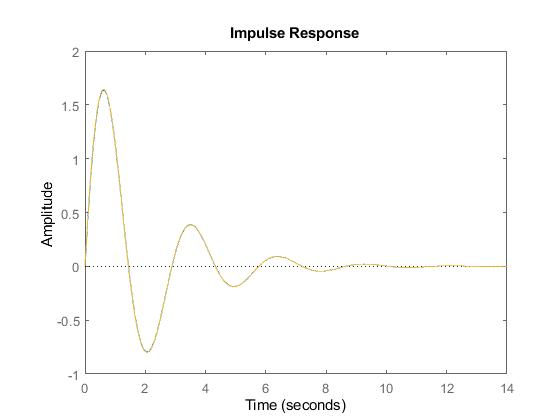
\includegraphics[width=0.7\linewidth]{SalidaTs00001DosHz}
	\caption{{Salida con $T_s=0.0001$}}
	\label{fig:salidaTs001-1}
\end{figure}

Debido a la gran aproximación de ambas gráficas se requiere de un acercamiento para poder observar las diferencias entre la gráfica generada con diferenciador (amarilla) y la generada sin diferenciador (roja).

\begin{figure}[H]
	\centering
	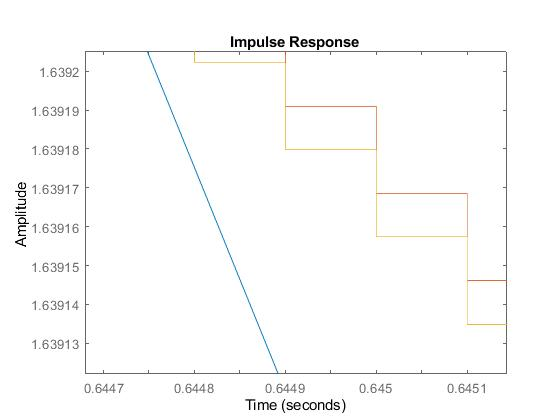
\includegraphics[width=0.7\linewidth]{SalidaTs00001DosHzAcercamiento}
	\caption{{Salida con $T_s=0.0001$}}
	\label{fig:salidaTs001-2}
\end{figure}

Gracias a este acercamiento podemos apreciar que la gráfica que se acerca más a la de tiempo continuo (azul) es la que utiliza un diferenciador (amarilla). Para esto utilizamos los comandos:

\begin{itemize}
\item Ts=0.0001
\item Hs=tf([5],[1 1 5])
\item Hz=c2d(Hs,Ts)
\item Hz2=c2d(Hs,Ts,'foh')
\item impulse(Hs)
\item hold on
\item dimpulse(Hz,Ts)
\item hold on
\item dimpulse(Hz2,Ts)
\end{itemize}

	\includepdf[pages={16}]{latex/practica3.pdf}
	\subsection{Solución actividad 4}

\subsubsection{Sistema 1}

Código en Matlab:

\begin{lstlisting}[language=Matlab]
x=0:10:620;
y= [32 33 34 36 38 39 40 40 40 40 39 39 39 37 37 38 38 38 38 38 38 39 38 38 38 38
38 38 38 38 38 38 38 38 38 38 38 38 38 38 38 38 38 38 38 38 38 38 38 38 38 38 38
38 38 38 38 38 38 38 38 38 38];

z= [1.6 1.7 1.8 1.9 2 2.1 2.17 2.135 2.137 2.328 2.117 2.103 2.094 1.95
1.98 2 2 2.01 2.07 2.067 2.065 2.085 2.07 2.067 2.065 2.064 2.062 2.06
2 2.056 2.055 2.052 2.05 2.048 2.05 2.052 2.055 2.055 2.055 2.049 
2.057 2.058 2.058 2.061 2.062 2.061 2.061 2.06 2.058 2.058 2.054
2.052 2.05 2.048 2.047 2.058 2.058 2.058 2.06 2.06
2.06 2.06 2.06];

plot(x,y,'b')
ylabel('Temperatura [c]')
xlabel('Tiempo [s]')
grid on

plot(x,z,'r')
ylabel('Voltaje [v]')
xlabel('Tiempo [s]')
grid on
\end{lstlisting}

Y ahora las gráficas anexadas como resultado del código.

\begin{figure}[H]
	\centering
	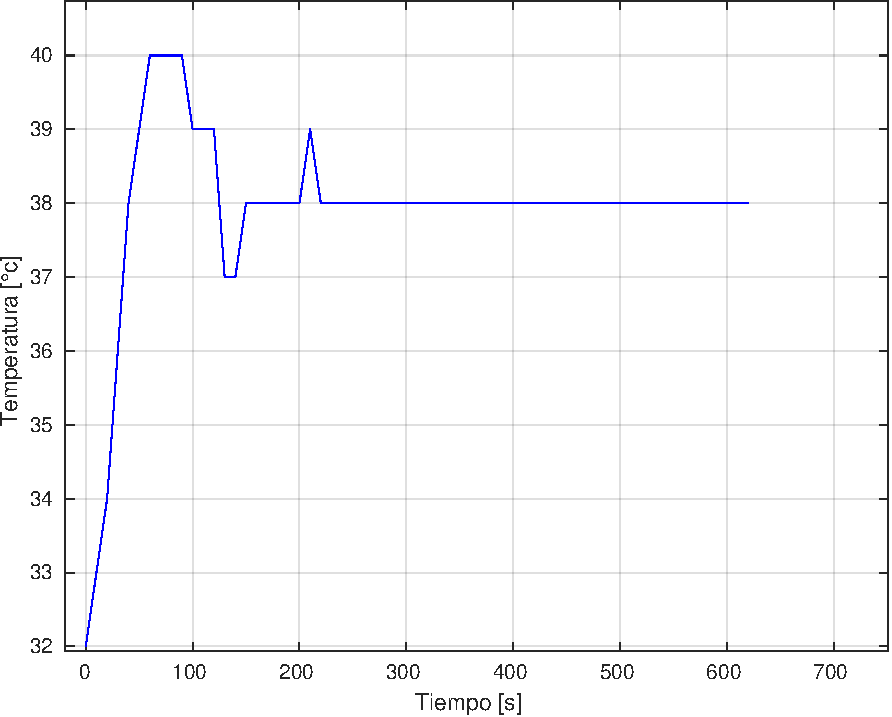
\includegraphics[width=0.7\linewidth]{img2/Grafica1}
	\caption{Gráfica de la temperatura vs tiempo}
	\label{fig:grafica1}
\end{figure}

\begin{figure}[H]
	\centering
	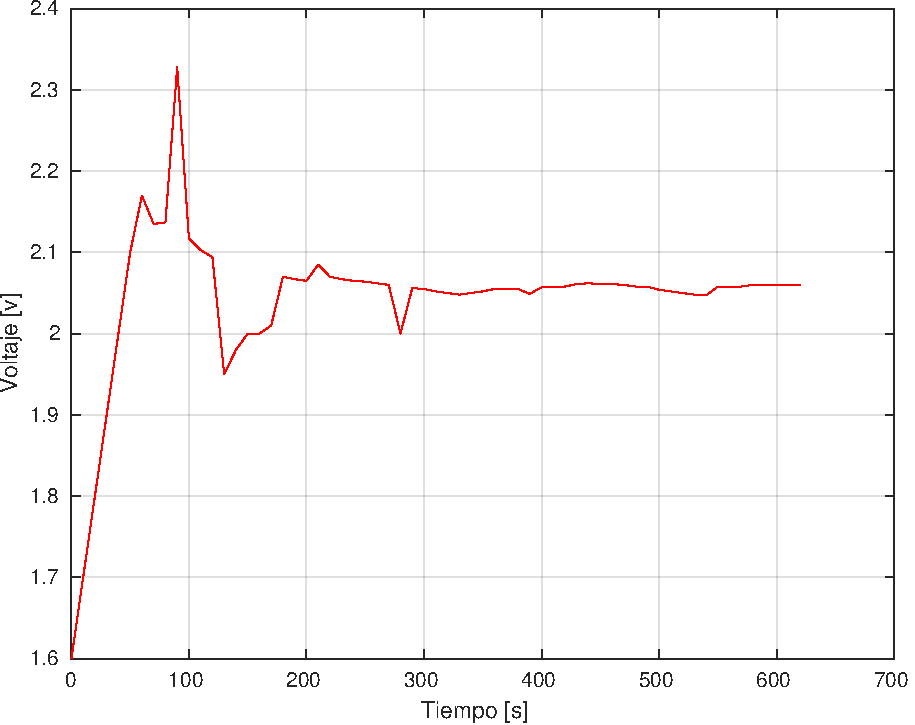
\includegraphics[width=0.7\linewidth]{img2/Grafica2}
	\caption{Gráfica del voltaje vs tiempo}
	\label{fig:grafica1}
\end{figure}

\textbf{3.-¿Cómo son las raíces del polinomio característicos del sistema de temperatura en estudio? justifique su respuesta.}

El comportamiento es sub-amortiguado, lo que quiere decir que primero tiene oscilaciones y después se estabiliza el sistema. $0<\zeta <1$ esta entre estos dos valores y por tanto las racies son complejas conjugadas de la forma:
$$-\zeta \omega_{n} \pm j \omega_{n} \sqrt{1-\zeta^{2}}$$

\textbf{4.-¿Las gráficas de voltaje y temperatura son continuas?}

Las gráficas son continuas, piense que la medición se usa tomando como eje x al tiempo y por tanto es continuo en ese eje. Si también se quiere decir que si la temperatura o el voltaje lo fueran, esto también se puede afirmar, ya que dichas mediciones su naturaleza es continua.
Como respuesta concreta, sí son continuas ambas gráficas.\\


\textbf{5.- ¿Cuál de las dos gráficas muestra mejor el comportamiento del sistema? Justifique su respuesta.}

La respuesta es algo subjetiva. Pienso que la gráfica de la temperatura muestra un mejor comportamiento sub-amortiguado, ya que las variaciones  para estabilizarse son menores y más predecibles que las variaciones del voltaje.



	\includepdf[pages={17}]{latex/practica3.pdf}
	\include{latex/pag17.tex}
	\includepdf[pages={18}]{latex/practica3.pdf}
	$$E(s)=R(s)-Y(s)$$
Donde: E(s) es el error medido, R(s) es la referencia y Y(s) es la salida.
$$H(s)=frac{Y(s)}{X(s)}$$
$$Y(s)=H(s)KX(s)$$
Si E(s)=X(s):
$$Y(s)=H(s)KE(s)$$
$$Y(s)=\frac{1}{s(s+3)}KE(s)$$
$$Y(s)=\frac{KE(s)}{s(s+3)}$$
$$E(s)=\frac{Y(s)(s(s+3))}{k}$$
Si $E(s)=R(s)-Y(s)$
$$R(s)-Y(s)=\frac{Y(s)(s(s+3))}{k}$$
$$KR(s)-KY(s)=Y(s)(s(s+3))$$
$$KR(s)=Y(s)(s(s+3)+K)$$
$$G_{c}(s)=\frac{Y(s)}{R(s)}=\frac{K}{s(s+3)+K}$$
Función de transferencia de lazo cerrado:
$$G_{c}(s)=\frac{Y(s)}{R(s)}=\frac{K}{(s(s+3)+K)}$$	
Si k=1:
$$G(s)=\frac{1}{(s(s+3)+1)}$$	
$$G(s)=\frac{1}{s^{2}+3s+1}$$	

\begin{figure}[H]
	\centering
	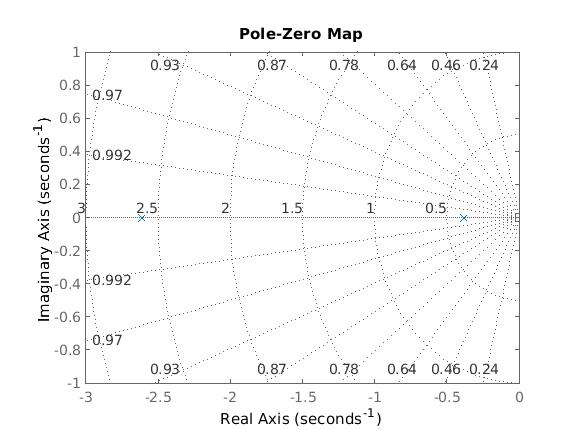
\includegraphics[scale=0.5]{G3.jpg}\
	\caption{{Si K=1}}
	\label{fig:salidaTs001-6}
\end{figure}
Polos: $P_{1}=-2.618$ y $P_{2}=-0.382$. Por lo tanto es estable el sistema.\\
Respuesta al escalón del sistema:\\

\begin{figure}[H]
	\centering
	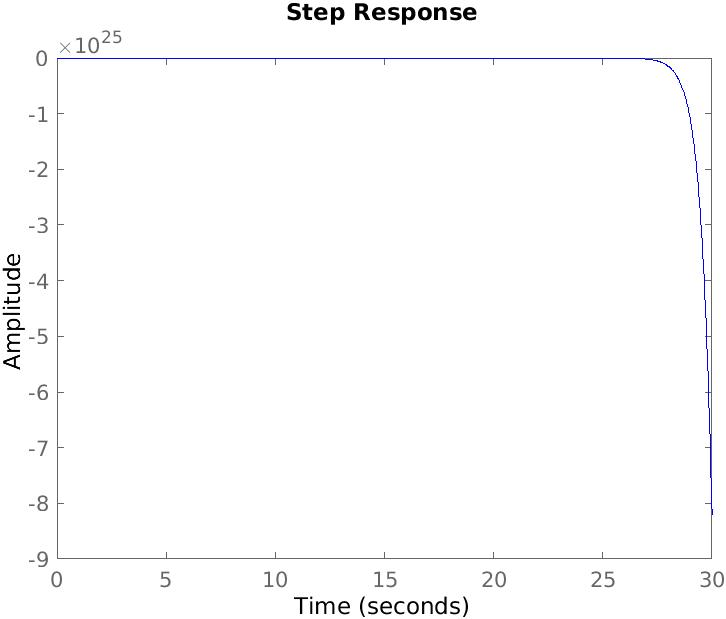
\includegraphics[scale=0.4]{G6.jpg}
	\caption{{Respuesta al escalón del sistema}}
	\label{fig:salidaTs001-6}
\end{figure}


Si k=-10:
$$G(s)=\frac{-10}{(s(s+3)-10)}$$	
$$G(s)=\frac{-10}{s^{2}+3s-10}$$

\begin{figure}[H]
	\centering
	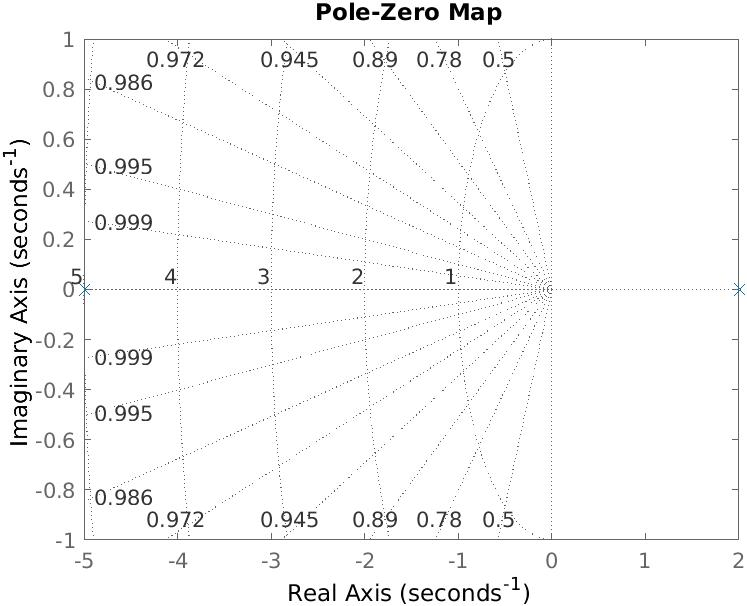
\includegraphics[scale=0.36]{G4.jpg}
	\caption{{Si K=-10}}
	\label{fig:salidaTs001-6}
\end{figure}


Polos: $P_{1}=-5$ y $P_{2}=2$. Por lo tanto es inestable el sistema.\\
Respuesta al escalón del sistema:

\begin{figure}[H]
	\centering
	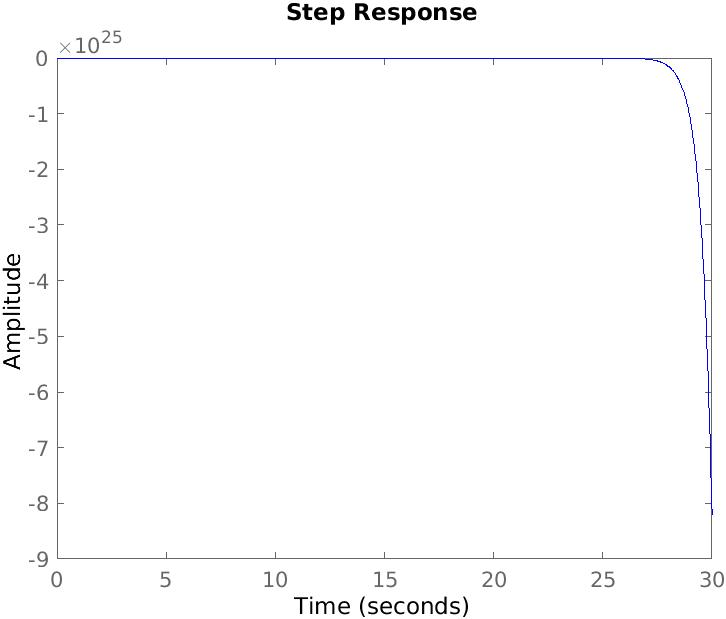
\includegraphics[width=0.4\linewidth]{G6.jpg}
	\caption{{Respuesta al escalón del sistema}}
	\label{fig:salidaTs001-7}
\end{figure}
	\includepdf[pages={19}]{latex/practica3.pdf}
	\include{latex/pag19.tex}
	\includepdf[pages={20-21}]{latex/practica3.pdf}
	\subsection{Solución actividad 5}
1. Identificar el numero de elementos que almacenan energía:\\
El sistema presenta cuatro almacenadores de energía. La ecuación resultante va a ser de orden dos, debido a que el sistema presenta los dos tipos de elementos almacenadores (de flujo y de esfuerzo), siendo estos elementos los siguientes:\\
\begin{itemize}
\item Almacenadores de esfuerzo: Inductores L y Lm
\item Almacenadores de flujo: Capacitor C y la masa rotada.
\end{itemize}
2. Identificar el número de restricciones físicas tanto de compatibilidad como de continuidad.\\
El sistema presenta cuatro restricciones físicas y se dividen de la siguiente forma: los dos circuitos en serie presentan restricciones de compatibilidad, mientras que la conexión en paralelo y la masa presentan restricciones de tipo de compatibilidad.\\
3. Plantear las restricciones físicas encontradas:\\
De la primera malla obtenemos el siguiente análisis:\\
\begin{equation}
E=V_L+v
\end{equation}
Si analizamos uno de los nodos que conecta a la primera malla con la conexión en paralelo obtenemos:\\
\begin{equation}
i=i_c+i_r+i_a
\end{equation}
De la segunda malla obtenemos el siguiente análisis:
\begin{equation}
v=V_{RM}+V_{LM}+VM
\end{equation}
Y por último, del sistema de la masa obtenemos lo siguiente:
\begin{equation}
K_{ew}=J\frac{d}{dt}w+Bw-J_L
\end{equation}
4. Sustituir las relaciones constitutivas de los elementos
Sustituyendo las relaciones constitutivas de los elementos de la primera malla obtenemos:
\begin{equation}
E=L\frac{d}{dt}i(t)+w
\end{equation}
En cuanto a los elementos constitutivos del análisis de la entrada de corriente al nodo alfa queda:
\begin{equation}
i=C\frac{dv}{dt}+\frac{v}{R}+i_a
\end{equation}
Y finalmente podemos expresar el análisis de la segunda malla de la siguiente forma:
\begin{equation}
v=R_mi_a+L_m\frac{d}{dt}i_a+K_{ew}
\end{equation}
5. Obtener el modelo matemático de forma matricial.
La representación del modelo matemático en forma matricial responde a la siguiente forma:
\begin{equation}
x'(t)=A(y)x(t)+B(t)u(t)
\end{equation}
La cual la podemos denotar como:
\begin{equation}
x'=Ax+Bu
\end{equation}
Donde $x'$ es el vector de variables de estados, $A$ es la matriz de estados, $x$ es el vector de estados, $B$ es la matriz de entrada y $u$ es el vector de entrada.\\
Para poder usar la expresión anterior debemos de dejar las ecuaciones de las restricciones de nuestro sistema en función de sus derivadas normalizadas. Po lo cual las ecuaciones a usar quedarán de las siguientes:
\begin{equation}
i'=-\frac{1}{L}v+\frac{1}{L}E
\end{equation}
\begin{equation}
v'=\frac{1}{C}i-\frac{1}{RC}v-\frac{1}{C}i_a
\end{equation}
\begin{equation}
i'_a=\frac{1}{L_m}v-\frac{1}{L_m}R_mi_a-\frac{K_e}{L_m}w
\end{equation}
\begin{equation}
w'=\frac{1}{J}k_ei_a-\frac{1}{J}B_w
\end{equation}
Ya teniendo las ecuaciones despejadas podemos sustituir en la ecuación matricial obteniendo la siguiente expresión:\\
llflfld
\begin{equation}
\begin{pmatrix}
i'\\
v'\\
i_a'\\
w' 
\end{pmatrix}
=
\begin{pmatrix}
0 & -\frac{1}{L} & 0 & 0\\
\frac{1}{C} & -\frac{1}{RC} & -\frac{1}{C} & 0\\
0 & \frac{1}{L_m} & -\frac{R_m}{L_m} & \frac{K_e}{L_m}\\
0 & 0 & \frac{K_e}{J} & -\frac{B}{J}
\end{pmatrix}
\begin{pmatrix}
i\\
v\\
i_a\\
w
\end{pmatrix}
+
\begin{pmatrix}
\frac{1}{L}\\
0\\
0\\
0\\
\end{pmatrix}
E
\end{equation}
6. ¿Qué se puede concluir del sistema físico obtenido?//
Que la unión de distintos sistemas físicos nos da como resultado la unión de las ecuaciones de dichos sistemas, es decir, su modelo matemático va a ser la suma de los modelos matemáticos de cada uno de los subsistemas que conforman a dicho sistema.

\section{OBSERVACIONES Y CONCLUSIONES}

	Villeda Hernandez Erick Ricardo: En la realización de esta práctica aplicamos los conocimientos teóricos de sobre el modelado de sistemas físicos (eléctricos, mecánicos translacional y mecánicos rotacionales), los cuales nos ayudaron a conocer y a diferenciar los elementos principales de todo sistema físico como los almacenadores de flujo, esfuerzo, los disipadores y la fuente de energía.Ya que dependiendo del tipo de sistemas con el que estemos trabajando va a variar su elementos. Se trabajó parte del funcionamiento de un sistema híbrido y se analizaron  las restricciones de constitución, continuidad, y compatibilidad para poder obtener un modelo matemático más apegado a la realidad.

	\nocite{webNijtEdu}
	\nocite{*}
	\bibliographystyle{plain}
	\bibliography{latex/referencias.bib}
\end{document}

